%========================================================================%
%               Copyright (C) 2016 All Rights Reserved.                  %
%             Author:BillHu<billhu@icloud.com>  Ver:<1.0>                %
%========================================================================%
%    The author grants permission, without fee and without a written     %
% license agreement, for use, reproduction, modification, and distribu-  %
% tion of this software and its documentation by educational, research,  %
% and non-profit entities for noncommercial purposes only.The above      %
% copyright notice and this paragraph MUST appear in all copies and      %
% modifications of the software and/or documentation.                    %
%========================================================================%
\documentclass{bjtuthesis}
%========================================================================%
% 自定义内容
%========================================================================%
\ctitle{基于边云融合的边缘云服务网格系统\\控制面子系统的设计与实现}
\etitle{The Design and Implementation of Intelligent Court Monitoring System Based on Video Recognition}
\cauthor{张璞}
\ctutor{刘海明}
\cschool{软件学院}
\cmajor{软件工程}
\category{工学}
\major{土木工程}
\cid{18301120}
\jobtitle{教授}
\degree{硕士}
\field{桥梁工程}
\cdata{2017年3月}
%========================================================================%
% 自定义文字
%========================================================================%
\cthanks{放置在摘要页前,对象包括:1)国家科学基金,资助研究工作的奖学金基金,合同单位,资助或支持的企业、组织或个人。2)协助完成研究工作和提供便利条件的组织或个人。3)在研究工作中提出建议和提供帮助的人。4)给予转载和引用权的资料、图片、文献、研究思想和设想的所有者。5)其他应感谢的组织和个人。}
\cabstract{[鼠标左键单击选择该段落,输入替换之。内容为小四号宋体。] 中文摘要应将论文的内容要点简短明了地表达出来,约400字左右,字体为宋体小四号。内容应包括工作目的、研究方法、成果和结论。要突出本论文的创新点,语言力求精炼。为了便于文献检索,应在本页下方另起一行注明论文的关键词(3-5个),如有可能,尽量采用《汉语主题词表》等词表提供的规范词。图X幅,表X个,参考文献X篇。}
\eabstract{[鼠标左键单击选择该段落,输入替换之。内容为小四号Times New Roman。] 与中文摘要内容要相对应。``the'' quick brown fox jumps over the lazy dog}
\cprelude{学位论文的序或前言,一般是作者或他人对本篇论文基本特征的简介,如说明研究工作缘起、背景、主旨、目的、意义、编写体例,以及资助、支持、协作经过等;也可以评述和对相关问题发表意见。这些内容也可以在正文引言中说明。}
\ckeywords{关键词1、关键词2、关键词3}
\ekeywords{KEYWORD1, KEYWORD2, KEYWORD3}
%========================================================================%
% 前置部分
%========================================================================%

\begin{document}

\pagenumbering{roman}
\cover

\ccopyright

\setcounter{page}{1}
% \ctitlepage
\pagestyle{myfancy}
\cabspage
% \myfanpage
\eabspage
% \myfanpage
% \cprepage
% \myfanpage

% \chapter*{目录}


\tableofcontents


\addcontentsline{toc}{part}{目\hspace{2em}录}%
\pagestyle{myfancy}
%========================================================================%
% 主体部份
%========================================================================%
% \markboth



\chapter{引言}
\pagestyle{myfancymain}
\setcounter{page}{1}
\pagenumbering{arabic}

[鼠标左键单击选择该段落,输入替换之。内容为小四号宋体。] 引言(或绪论)简要说明研究工作的目的、范围、相关领域的前人工作和知识空白、理论基础和分析、研究设想、研究方法和实验设计、预期结果和意义等。应言简意赅,不要与摘要雷同,不要成为摘要的注释。一般教科书中有的知识,在引言中不必赘述。
\chapter{【1级标题,三号黑体字】}
 [鼠标左键单击选择该段落,输入替换之。内容为小四号宋或楷体字。] 学位论文为了需要反映出作者确已掌握了坚实的基础理论和系统的专门知识,具有开阔的科学视野,对研究方案作了充分论证,因此,有关历史回顾和前人工作的综合评述,以及理论分析等,可以单独成章,用足够的文字叙述。正文是学位论文的核心部分,占主要篇幅,可以包括:调查对象、实验和观测方法、仪器设备、材料原料、实验和观测结果、计算方法和编程原理、数据资料、经过加工整理的图表、形成的论点和导出的结论等。\par
由于研究工作涉及的学科、选题、研究方法、工作进程、结果表达方式等有很大的差异,对正文内容不能作统一的规定。但是,必须实事求是,客观真切,准确完备,合乎逻辑,层次分明,简练可读。\par
\textcolor{red}{\textbf{图:}}\par
图包括曲线图、构造图、示意图、框图、流程图、记录图、地图、照片等。\par
图应具有“自明性”。\par
图应有编号。图的编号由“图”和从“1”开始的阿拉伯数字组成,图较多时,可分章编号。\par
图宜有图题,图题即图的名称,置于图的编号之后。图的编号和图题应置于图下方。\par
照片图要求主题和主要显示部分的轮廓鲜明,便于制版。如用放大缩小的复制品,必须清晰,反差适中。照片上应有表示目的物尺寸的标度。\par
图片示例1:
\begin{figure}[!htp]
    \centering
    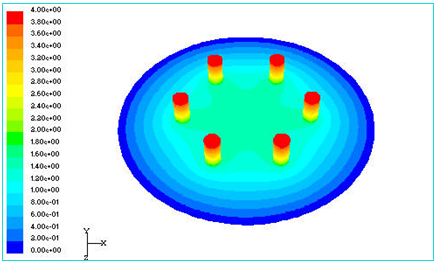
\includegraphics[width=0.5\textwidth]{pic/pic2-1.png}
    \caption{太合金多炭钢铁产品柱扭曲局部受力分析示意图\label{fig:2-1}}
\end{figure}

\textcolor{red}{\textbf{表:}}\par
表应具有“自明性”。\par
表应有编号。表的编号由“表”和从“1”开始的阿拉伯数字组成,表较多时,可分章编号。表较多时,可分章编号。表较多时,可分章编号。表较多时,可分章编号。\par
表宜有表题,表题即表的名称,置于表的编号之后。表的编号和表题应置于表上方。\par
表的编排,一般是内容和测试项目由左至右横读,数据依序竖读。\par
表的编排建议采用国际通行的三线表。\par
如某个表需要转页接排,在随后的各页上应重复表的编号。编号后跟表题(可省略)和“(续)”,置于表上方。\par
续表均应重复表头。\par
表格示例1:

\begin{table}[htbp]
    % \zihao{5}\mysongti

    \centering
    \caption{国际单位制的基本单位}
    \label{tbl:2-1}
    \begin{tabularx}{0.8\textwidth}{*{3}{>{\centering\arraybackslash}X}}
        \toprule
        量的名称   & 单位名称     & 单位符号 \\ \midrule
        长度       & 米           & m        \\
        质量       & 千克(公斤)   & kg       \\
        时间       & 秒           & s        \\
        电流       & 安{[}培{]}   & A        \\
        热力学温度 & 开{[}尔文{]} & K        \\
        物质的量   & 摩{[}尔{]}   & mol      \\
        发光强度   & 坎{[}德拉{]} & cd       \\ \bottomrule
    \end{tabularx}
\end{table}

\textcolor{red}{\textbf{公式:}}\par
论文中的公式应另行起,并缩格书写,与周围文字留足够的空间区分开。\par
如有两个以上的公式,应用从“1”开始的阿拉伯数字进行编号,并将编号置于括号内。公式的编号右端对齐,公式与编号之间可用“…”连接。公式较多时,可分章编号。\par
公式示例1:
\begin{equation}
    \label{eqn:2}
    \phi=\frac{D_{p}^{2}}{150} \frac{\psi^{3}}{(1-\psi)^{2}}
\end{equation}
\begin{equation}
    \label{eqn:3}
    C_{2} =\frac{3.5}{D_{p}} \frac{(1-\psi)}{\psi^{3}}
\end{equation}

\noindent 式中  $\quad D_{p}$ —— 多孔质材料的平均粒子直径($m$);\par
$\psi$ —— 孔隙度(孔隙体积占总体积的百分比); \par
$\phi$ —— 特征渗透性或固有渗透性,与材料的结构性质有关($m^2$)。\par
较长的公式需要转行时,应尽可能在“=”处回行,或者在“+”、“-”“×”、“/”等记号处回行。\par
公式中分数线的横线,其长度应等于或略大于分子和分母中较长的一方。\par
如正文中书写分数,应尽量将其高度降低为一行。如将分数线书写为“/”,将根号改为负指数。\par
公式示例2:\par
\begin{spacing}{2}
    \begin{math}
        \zihao{5} \quad\text{将}\;\dfrac{1}{\sqrt{2}}\;\text{写成}\; 1/\sqrt{2} \;\text{或}\; 2^{-1/2}。
    \end{math}
\end{spacing}

\textcolor{red}{\textbf{引文标注}}\par
论文中引用的文献的标注方法遵照GB/T 7714-2005,可采用顺序编码制,也可采用著者-出版年制,但全文必须统一。\par
\textcolor{red}{\textbf{注释}}\par
当论文中的字、词或短语,需要进一步加以说明,而又没有具体的文献来源时,用注释。注释一般在社会科学中用得较多。\par
应控制论文中的注释数量,不宜过多。\par
由于论文篇幅较长,建议采用文中编号加“脚注”的方式。最好不用采用文中编号加“尾注”。\par

\section{【2级标题,小三号黑体字】 }
 [鼠标左键单击选择该段落,输入替换之。内容为小四号宋或楷体字。]
\subsection{【3级标题,四号黑体字】 }
[鼠标左键单击选择该段落,输入替换之。内容为小四号宋或楷体字。]

\chapter{【1级标题,三号黑体字】}
\section{【2级标题,小三号黑体字】 }
 [鼠标左键单击选择该段落,输入替换之。内容为小四号宋或楷体字。]
\subsection{【3级标题,四号黑体字】 }
[鼠标左键单击选择该段落,输入替换之。内容为小四号宋或楷体字。]

\chapter{【1级标题,三号黑体字】}
\section{【2级标题,小三号黑体字】 }
 [鼠标左键单击选择该段落,输入替换之。内容为小四号宋或楷体字。]
\subsection{【3级标题,四号黑体字】 }
[鼠标左键单击选择该段落,输入替换之。内容为小四号宋或楷体字。]

\chapter{结论【1级标题,三号黑体字】 }
 [鼠标左键单击选择该段落,输入替换之。内容为小四号宋或楷体字。] 论文的结论是最终的、总体的结论,不是正文中各段的小结的简单重复。结论应该准确、完整、明确、精练。如果不可能导出应有的结论,也可以没有结论而进行必要的讨论。可以在结论或讨论中提出建议、研究设想、仪器设备改进意见以及尚待解决的问题等。

\chapter{各种测试}
\section{图表测试}
\subsection{单张图片}
单张普通插图,及其引用,如图\ref{fig:G1}所示。

\begin{figure}[!htp]
    \centering
    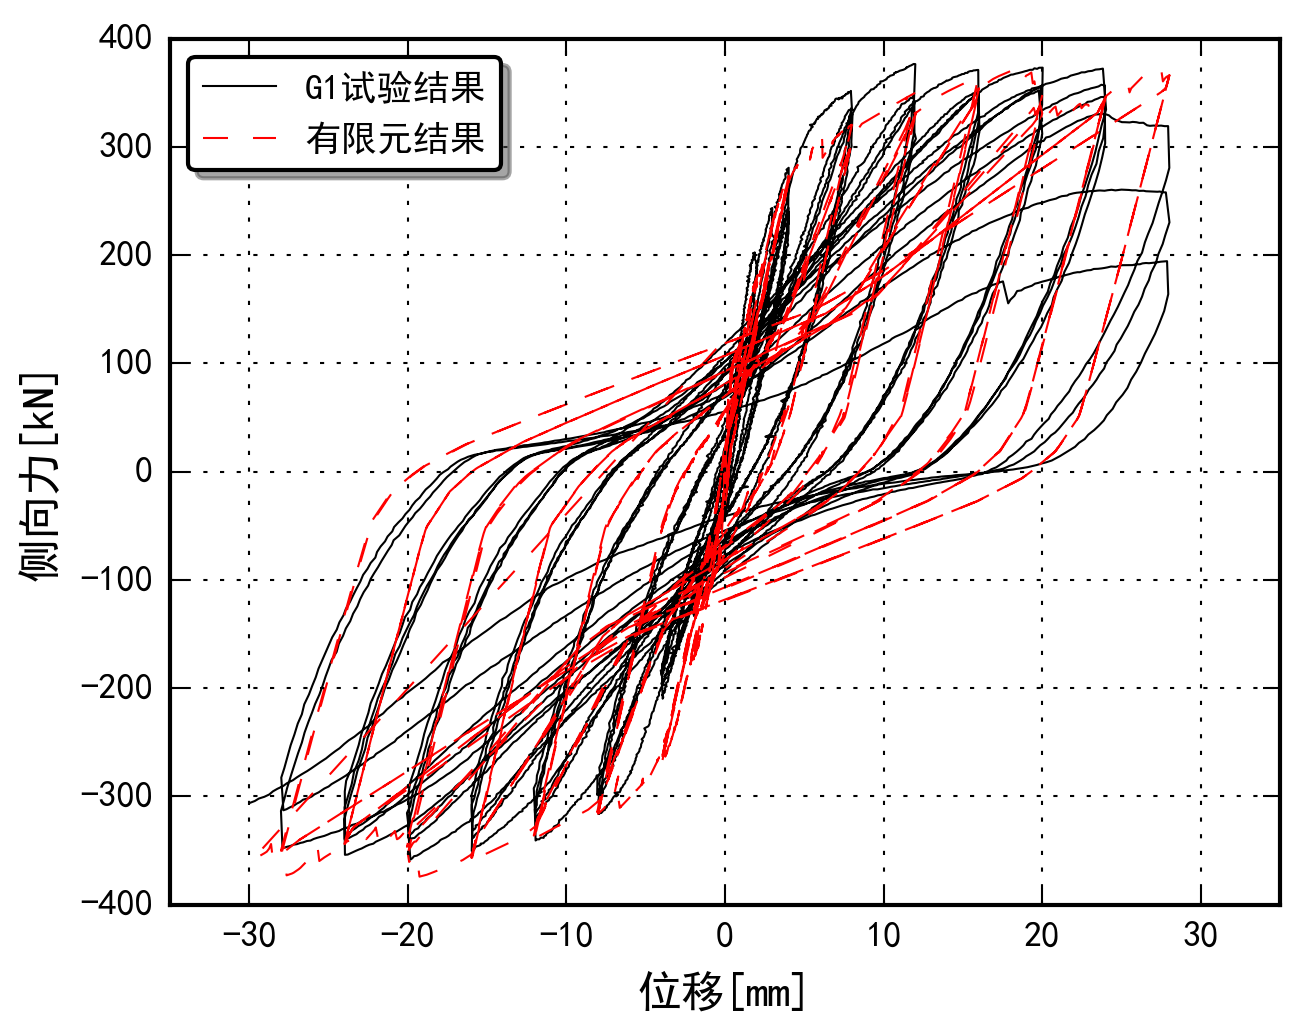
\includegraphics[width=0.8\textwidth]{pic/G1.png}
    \figcaption{G1数据对比\label{fig:G1}}{Comparison of experimental data}
\end{figure}

\subsection{多张图片}
多张图片联排或者换行可以使用各种排版方式(minipage、subplot等),如下图\ref{fig:2}所示。
\begin{figure}
    \centering
    \begin{minipage}[t]{0.48\textwidth}
        \centering
        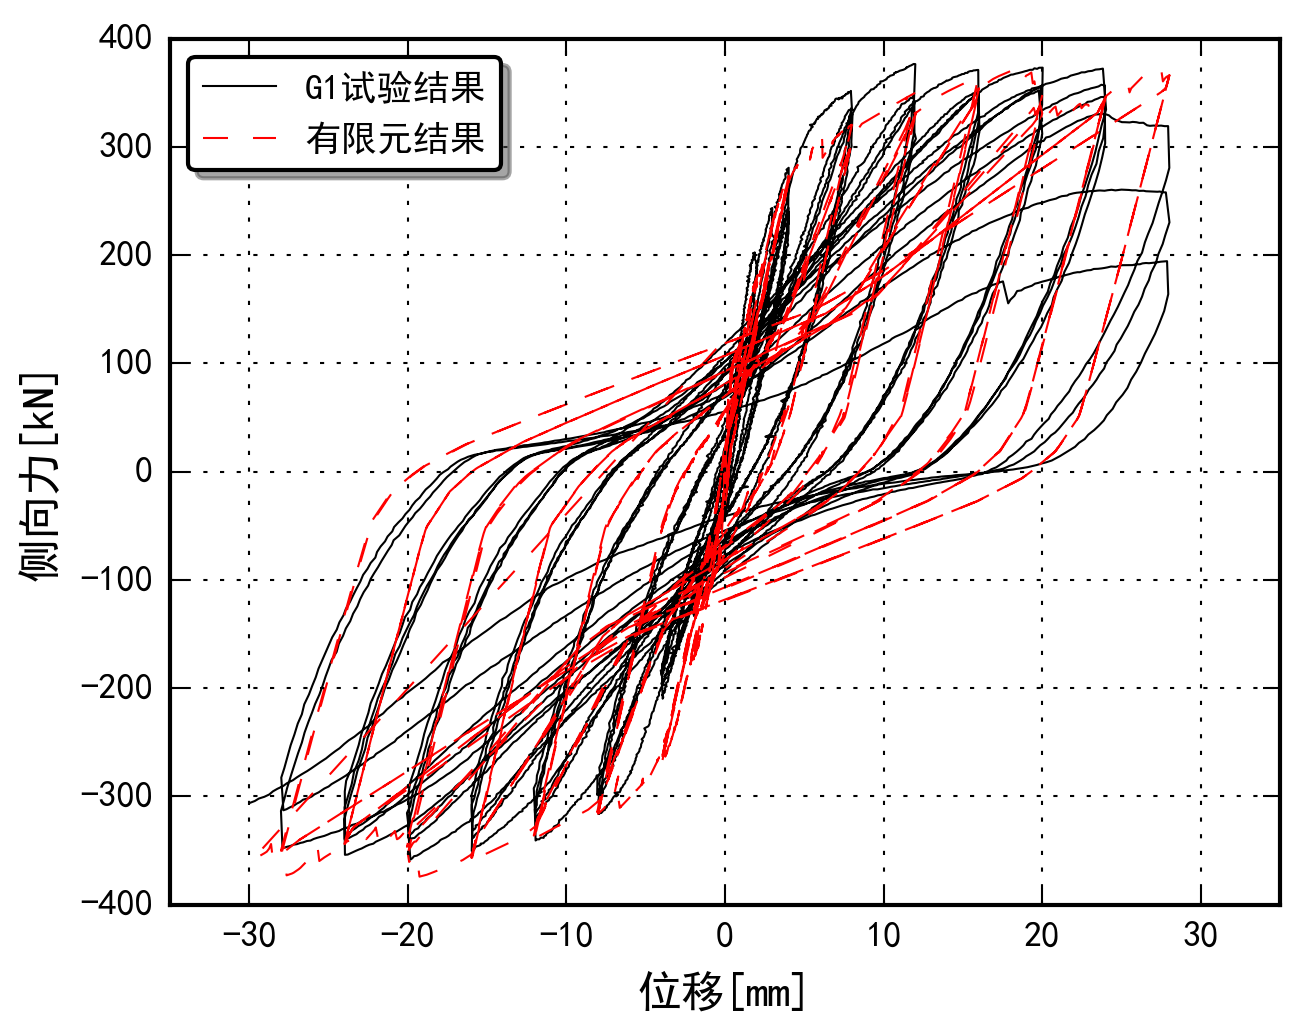
\includegraphics[width=0.9\textwidth]{pic/G1.png}\\
        {\zihao{5}(a) G1试件}
    \end{minipage}
    \begin{minipage}[t]{0.48\textwidth}
        \centering
        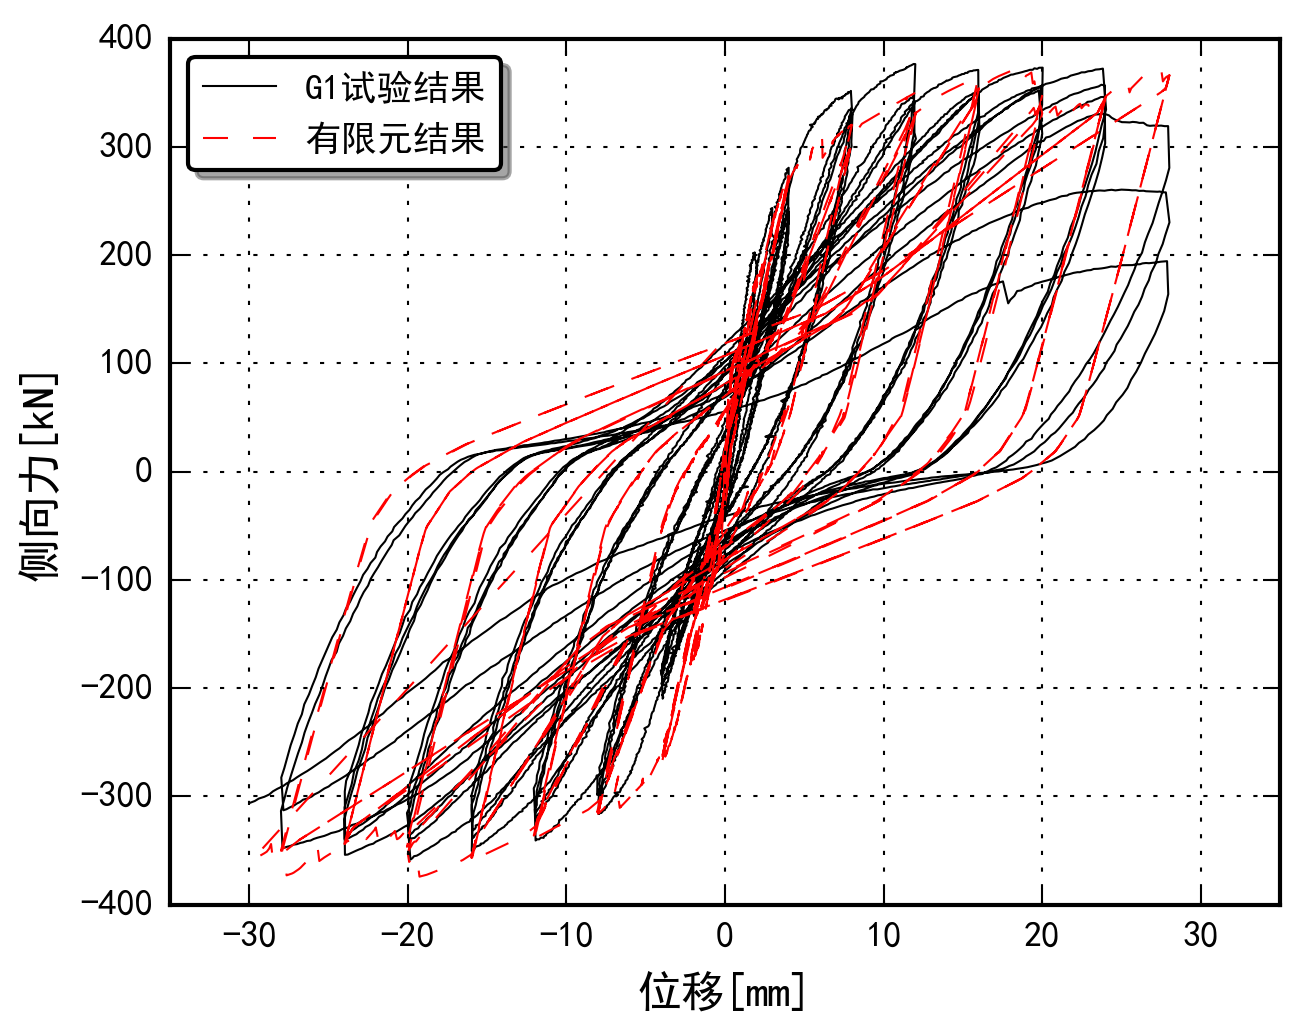
\includegraphics[width=0.9\textwidth]{pic/G1.png}\\
        {\zihao{5}(b) G1试件}
    \end{minipage}
    \figcaption{太合金多炭钢铁产品柱扭曲局部受力分析示意图\label{fig:2}}{Comparison of experimental data}
\end{figure}
\section{公式测试}
公式的排版和引用与正常\LaTeX\ 公式格式一致。例如:

\begin{equation}
    \label{eqn:1}
    e^{i\pi}+1=0
\end{equation}

欧拉公式(式\ref{eqn:1}),它是数学里最令人着迷的一个公式,它将数学里最重要的几个数学联系到了一起——两个超数:自然对数的底$e$,圆周率$\pi$;两个单位:虚数单位$i$和自然数的单位$1$,以及数学里常见的$0$。数学家们评价它是“上帝创造的公式”,我们只能看它而不能理解它。

\section{参考文献测试}
我使用的参考文献是符合《GB7714-2005》规范的中文论文参考文献格式。该规范作为国家标准化管理委员会正式公布的标准,其权威性和通用性远远超过了其它格式规范,是国内最正式的参考文献格式规范,并且是大多数高校毕业论文和杂志的指定参考文献格式。

下面分类测试各种类型参考文献:

\begin{itemize}
    \item 中文规范\citep{C1}。
    \item 英文规范\citep{ACI318}
    \item 中文学位论文\citep{liguiqian}
    \item 英文学位论文\citep{bentz2000}
    \item 期刊\citep{FMK}
    \item 图书类\citep{B1}
    \item 其他\citep{R1}
    \item 多文献引用,压缩格式\citep{C1,ACI318,liguiqian,R1}
\end{itemize}

\chapter{结论}
论文的结论是最终的、总体的结论,不是正文中各段的小结的简单重复。结论应该准确、完整、明确、精练。如果不可能导出应有的结论,也可以没有结论而进行必要的讨论。可以在结论或讨论中提出建议、研究设想、仪器设备改进意见以及尚待解决的问题等。
%========================================================================%
% 参考文献
%========================================================================%


% \bibliography{MyDissBib}

\newpage
\pagestyle{myfancy}
\nocite{*}
\printbibliography[heading=myheading]
\addcontentsline{toc}{part}{参考文献}
\cleardoublepage
%========================================================================%
% 附录
%========================================================================%
\thankspage
\markboth{附录}{}
\addcontentsline{toc}{part}{附\hspace{2em}录}
\begin{center}
    {\zihao{3}\heiti 附录A}
\end{center}
\begin{center}
    {\zihao{3}\heiti 附录标题}
\end{center}

% \indent\zihao{5}附录是作为论文主体的补充项目,并不是必须的。
% 论文的附录依序用大写正体英文字母A、B、C……编序号,如:附录A。
% \cleardoublepage
% %========================================================================%
% % 索引
% %========================================================================%
% \markboth{索引}{}
% \addcontentsline{toc}{part}{索引}
% \begin{center}
%     {\zihao{3}\heiti 索引}
% \end{center}

% \indent\zihao{5}按照需要编排分类索引、著者索引、关键词索引等。
% \cleardoublepage
% %========================================================================%
% % 作者简历及研究成果
% %========================================================================%
% \markboth{作者简历及攻读硕士学位期间取得的研究成果}{}
% \addcontentsline{toc}{part}{作者简历及攻读硕士学位期间取得的研究成果}
% \begin{thecenter}
%     作者简历及攻读硕士学位期间取得的研究成果
% \end{thecenter}

% \zihao{5}包括教育经历、工作经历、攻读学位期间发表的论文和完成的工作等。行距16磅,段前后各为0磅。
\cleardoublepage
% \cstatement
% \clastpage
\end{document}
